\section{Densite de force associe a la pression}\todo{Lecture 3}

Calculons la force exercee sur un volume de fluide infinitessimal due a la pression. On suppose que $p=p(\boldsymbol{r})$ est arbitraire:

On note $\boldsymbol{F}_{1}=p\left( -\frac{dx}{2},0,0\right)dydz~\boldsymbol{e}_{x}$ et $\boldsymbol{F}_{2}=-p\left( \frac{dx}{2},0,0 \right)dydz~\boldsymbol{e}_{x}$ donc on a 
\begin{align*}
\sum \boldsymbol{F}_{i} & =\left( p\left( -\frac{dx}{2},0,0 \right)dydz-p\left( \frac{dx}{2},0,0 \right)dydz \right)~\boldsymbol{e}_{x} +\dots\\
 & =-\frac{p\left( \frac{dx}{2},0,0 \right)-p\left( -\frac{dx}{2},0,0 \right) }{dx}dxdydz~\boldsymbol{e}_{x}+\dots \\
 & =-\frac{ \partial p }{ \partial x } dV~\boldsymbol{e}_{x}+\dots \\
 & =-\boldsymbol{\nabla}_{p}dV
\end{align*}

alors la densite est forme associe a la pression $-\boldsymbol{\nabla}_{p}$.

\begin{example}
Sur un volume $V$ de surface $S$ on peut calculer la force de pression sur $V$:
$$
\boldsymbol{F}_{p}=\underset{n\to \infty}{\lim_{ |\Delta \boldsymbol{S}_{i}| \to 0 } }\sum_{i=1}^{n} -p(\boldsymbol{r}_{i})\Delta \boldsymbol{S}_{i}=-\iint _{S}p~d\boldsymbol{S}
$$
ou de maniere alternative en utilisant $-\boldsymbol{\nabla}_{p}$:
$$
\boldsymbol{F}_{p}=\iiint _{V}-\boldsymbol{\nabla}_{p}~dV
$$

Maintenant soit $p=p_{0}-\rho gz$ pour $z\le 0$, on voit que :
\begin{align*}
\boldsymbol{F}_{p} & =-\iint p~d\boldsymbol{S}=\iiint-\boldsymbol{\nabla}_{p}~dV \\
 & =\iint _{V}-\boldsymbol{\nabla}(p_{0}-\rho gz)~dV \\
 & =\iint _{V}\rho g~\boldsymbol{e}_{z}~dV \\
 & =\rho g\iint _{V}dV~\boldsymbol{e}_{z}=\rho gV~\boldsymbol{e}_{z}=mg~\boldsymbol{e}_{z} 
\end{align*}
\end{example}

Ce resultat est valable meme si le volume $V$ est par exemple un solide.
\begin{proposition}[Pousee d'Archimede]
Tout corps plongee dans un fluide recoit de la part de celui-ci une pousee verticale egale au poids du fluide deplace.
\end{proposition}

\begin{example}
\section{Tension superficielle}
\begin{figure*}[h!]
\centering
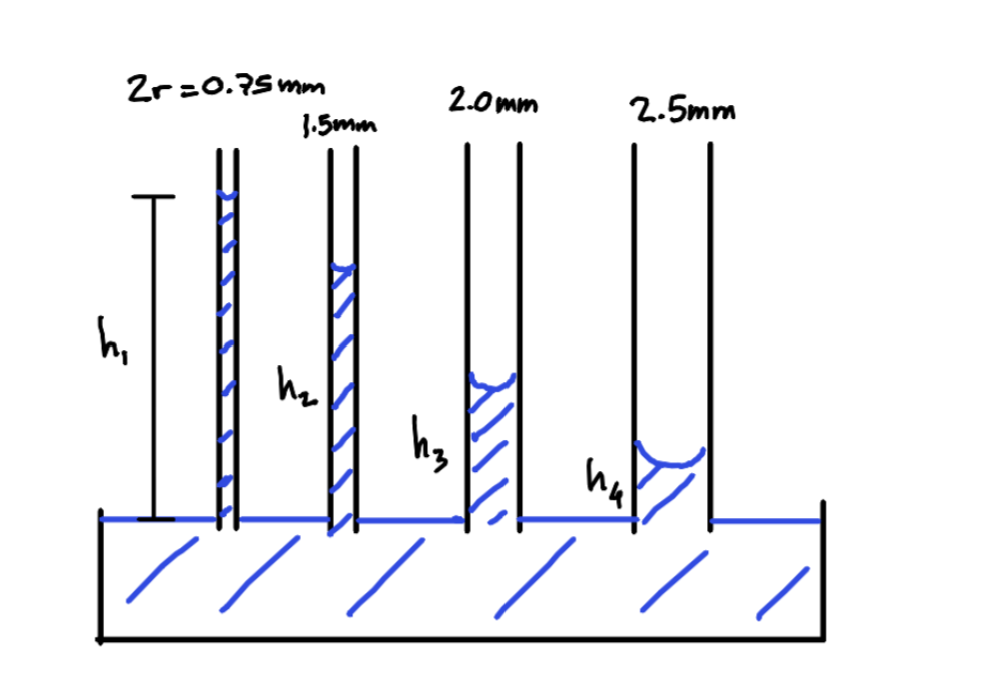
\includegraphics{test}
\end{figure*}
Ou $h_{1}=34\mathrm{mm}$, $h_{2}=17\mathrm{mm}$, $h_{3}=13\mathrm{mm}$ et $h_{4}=10\mathrm{mm}$.
\end{example}

\begin{question}
Contradiction avec $p(h)=\rho p_{0}gh$?
\end{question}
\begin{answer}
Non, on verra que ce phenomene du a la tension superficielle et $p=p_{0}\rho gh$ reste valable a l'interieur du fluide.
\end{answer}
\subsection{Definition et origine de la tension superficielle}
\begin{example}
Soit un filon de liquide (p.ex. de l'eau savonneuse) tendu dans un cadre forme de sommets $ABCD$. 
\begin{figure}[h!]
\centering
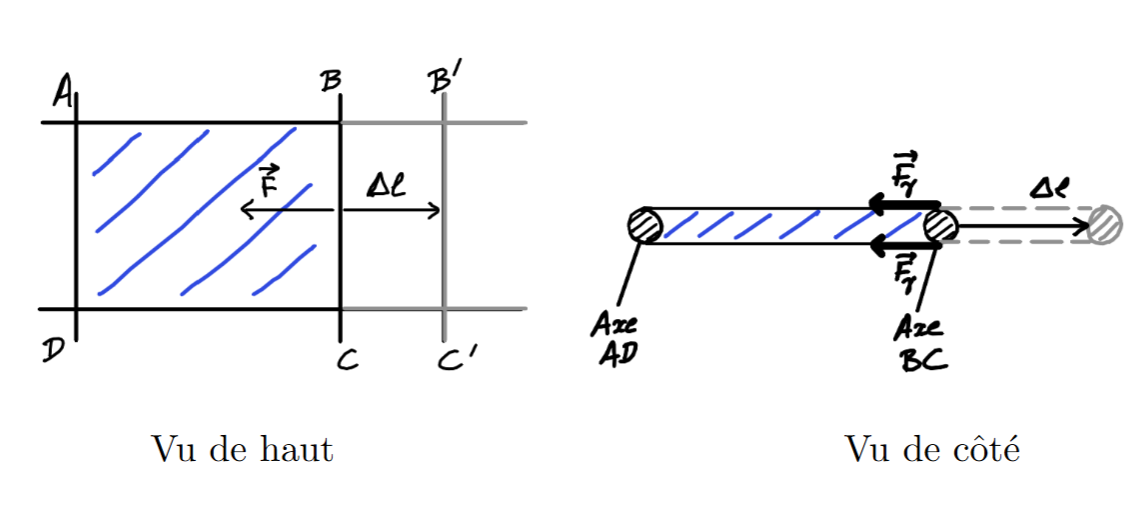
\includegraphics{cadreau}
\end{figure}
Pour deplacer $\boldsymbol{BC}$ a $\boldsymbol{B}'\boldsymbol{C}'$ il faut faire un travail $$\Delta W\propto \Delta S=\gamma\Delta S=2\cdot\gamma\cdot \boldsymbol{BC}\cdot\Delta \ell$$ ou $\Delta S$ est le changement de surface du liquide/gaz, $\gamma$ est la tension superficielle, qu'on mesure en newton-metre $[\gamma]=\mathrm{N}\mathrm{m}^{-1}$.

Comme en generale on a que $\Delta W=\boldsymbol{F}\Delta \boldsymbol{\ell}$ on a que $\boldsymbol{F}=2\boldsymbol{F}_{\gamma}=2\gamma \boldsymbol{BC}$ ou $\boldsymbol{F}_{\gamma}$ est la force tangentielle a la surface et perpendiculaire a son bord.
\end{example}
\begin{example}
\begin{figure}[h!]
\centering
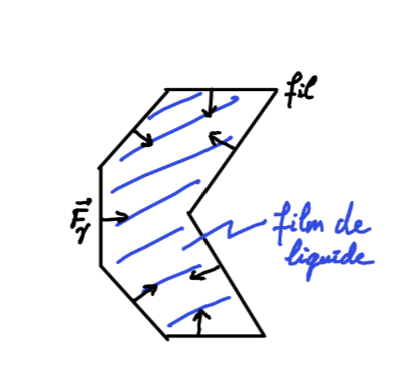
\includegraphics{exa1}
\end{figure}
\end{example}
\begin{remark}
L'interface liquide/gaz est un peu comme une membrane elastique, mais la force est independante de la deformation.
\end{remark}
\begin{question}
Quel est l'origine microscopique de cette force?
\end{question}
\begin{answer}
Ils existent des liaisons intermoleculaires dans un fluide:
\begin{itemize}
\item Interactions intermoleculaires: attraction de Van der Waals, liasons de hydrogene.
\item Repulsion a petite distance due au principe de Pauli.
\end{itemize}
mais il y'a moins de ces liaisons par molecule a la surface du liquide. Pour l'amener la-bas et agrandir la surface, il faut faire un travail ! (pour "briser" ces liaisons)
\end{answer}
\begin{example}[Mesure de $\gamma$]
Tensiometre p.23 poly
\end{example}

Certaines consequences immediates de la tension superficielle:
\begin{itemize}
\item Bulles de savon minimisent leur surface $\Rightarrow$ sphere.
\item Meme chose pour les bulles d'eau en apesanteur. 
\item Les cheveux mouilees qui collent (mais pas sous l'eau).
\item Certains obejtes (trombone, punaise) ou insectes qui flottent.
\end{itemize}
\begin{example}[Bateau a savon]
Ajouter du savon a la surface de l’eau autour de l’arriere du bateau diminue $\gamma$ dans cette region,
ce qui genere une force nette : le bateau se met alors a bouger.
\end{example}
